A program működése 2 részre bontható: weboldalra(kliens) és a szerverre.
A weboldalon össze állított adatokat küldjük fel a szerverre, a szerver a megkapott adatok alapján számol. \newline
\subsection{Weboldal}
	A kliens megvalósításához az alábbi technológiák merültek fel : C++/Qt, C\#, JS/HTML. Végül JavaScript-ben lett megvalósítva, első sorban a grafikon kirajzoló (Flot) miatt, de a szerver kommunikáció egyszerűsége is döntő ok volt amellett, hogy egy weboldal bármely gépen egyszerűen megnyitható, kezelhető.\newline
	Egy oldalból áll melyen a felhasználó szerkesztheti az adatokat. Azért nem lettek a részek külön oldalakon megvalósítva, mert az egyik oldalról az adatok átvitele egy másik oldalra nem annyira egyszerű, viszont nincs is olyan komplex az oldal, hogy szükséges legyen több aloldalra szétbontani. 
	Az oldal megjelenés felépítése megtekinthető \ref{fig:weblap_vazlat}-es képen.
	\begin{figure}[h]
	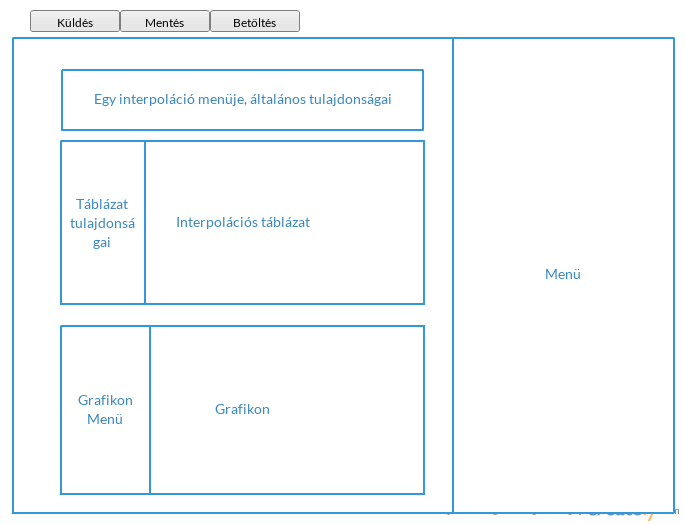
\includegraphics[width=14cm]{pics/weblap_vazlat}
	\centering
	\caption{Weboldal vázlata\label{fig:weblap_vazlat}}
	\end{figure}
	Az első döntés, melyet a felülettel kapcsolatban meg kellett hozni a kirajzolás módja. Mivel JavaScript-hez találtam egy gyorsan megtanulható és kényelmes grafikon kirajzolót, ezért végül webes kliens mellett döntöttem. A grafikon kirajzolóról a \ref{subsec:flot} pontban lehet olvasni.
	A weboldalon meg kell valósítani a pontok dinamikus kirajzolását, és a táblázatos formában történő megjelenítést és szerkeszthetőséget. Mivel több interpolációt küldünk fel a szervernek ezért a weboldalon több szerkesztésére is lehetőséget kell adni. \newline 
	Több interpoláció számítás szerkesztésének megvalósításához kell egy menü rendszer, amelyben eltárolódnak az adatok, és képesek betöltődni.\newline
	Az oldalon input-okat használunk még, és a dinamikus táblázat is JavaScript-ből van legenerálva. A táblázatokban sorok beszúrására teljes táblázat törlésre is lehetőséget kell adni. 
	A táblázatokban inputok vannak az egyes cellákban melyben egyszerű értékek, vagy akár komplexebb Objektumok is találhatóak. A bonyolultabb objektumokat json string-ben tároljuk ezekben az inputokban. \newline
	A menü listájában új adathalmazokat hozhat létre, a régieket szerkesztheti.
	Amikor a felhasználó pontokat, megjelenítést frissít a legtöbb esetben az oldal már a háttérben menti az adatokat a listába. Amikor egy másik interpolációt választunk ki, akkor az betöltődik a táblázatba, és a grafikonba. A módosítások és mentés esetén az aktuálisan kiválasztott interpolációs adathalmaz sora fog frissülni.
	Ha a felhasználó végzett egy gombra nyomással a program legenerálja a szükséges objektumot. \newline
	A felület sok gombot tartalmaz, melyek hatására frissíthetőek az adatok. Amikor frissítünk egy részt, általában mentődnek az értékek egy inputba JSON formában.

\subsection{Elosztott rendszer}
	Az elosztott rendszer megvalósításához az alábbi technológiák merültek fel: \newline C++/PVM, Erlang.
	Miután a JavaScript mellett döntöttem a grafikus felületen, ezután optimálisabbnak tűnt egy hasonlóan gyengén típusos nyelvnek a használata. Az Erlang elég jól támogatja párhuzamosítást és a szerver kommunikációt is, és bár az algoritmusok implementálása nehézkesebb lett volna, de C++-ban megvalósított függvények beépítése miatt ez a probléma megoldódott.
	\newline
	A JavaScript-ből kapott json kibontására talált mochijson segítségével az adatokat át lehetett dolgozni Erlang-os típusokká, alkalmazásáról a \ref{subsec:mochijson} pontban lesz szó.

\subsection{Számítás}
	A számítás megvalósításánál felmerült hogy Erlang-ban legyen, de mivel a számítást ciklusokkal érdemes megvalósítani, ezért egyszerűbb volt egy nem funkcionális nyelvben implementálni azokat.
	A C++-os függvényeket fel lehetett használni az Erlang modulokban. Erre a NIF könyvtárat használtam, melyről az \ref{subsec:nif} pontban részletesen szó esik. 
\subsection{Kommunikáció}
	Amikor a szervert létrehozzuk akkor inicializálunk két processzt. Az egyik a kliens felől várakozik kérésre, a másik a node-ok felől. Amikor egy node fel kíván csatlakozni, küld egy kérést. Ha sikeres volt akkor a szerver ezt jelzi neki, és felkerül a listára. \newline
	A weboldalon egy gomb hatására megy egy kérés a szerver felé. A szerver jó esetben fogadja a kérést. Ha a kliensnek nem sikerült kapcsolatba lépnie a szerverrel, akkor jelzi a felhasználónak hogy a kapcsolódás során hiba lépett fel. \newline
	Ha fogadta a kérést, akkor megpróbálja feldolgozni az adatokat. Ha sikeresen feldolgozta az adatokat, abban az esetben elindul a szétosztás. \newline
	A szétosztás során a felcsatlakozott gépeken létre jönnek a processzek, majd kapnak egy adathalmazt mellyel számolniuk kell. Ha végeztek, az eredményt visszaküldik a szülő processznek. A szülő processz, ha megkapott minden értéket, azt visszaküldi a weboldalnak.
	\newline
	A weboldal sikeres válasz után betölti az eredményeket. 
	\begin{figure}[h]
		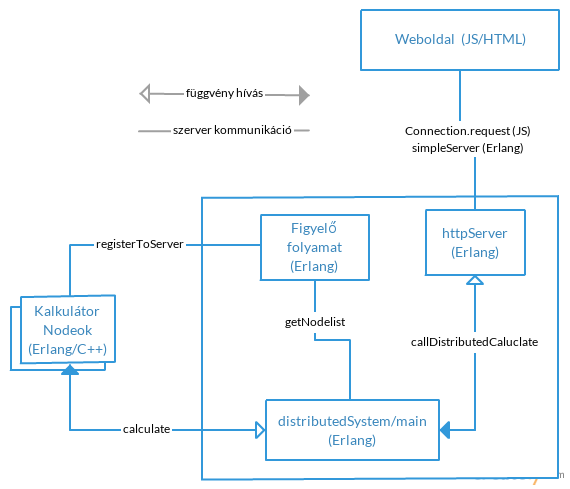
\includegraphics[width=13cm]{pics/kommunikacio1}
	\centering
	\caption{Kommunikáció\label{fig:kommunikacio1}}
	\end{figure}